\documentclass[preprint,12pt]{elsarticle}

\usepackage{amsmath,amssymb,amsfonts}
\usepackage{graphicx}
\usepackage{booktabs}
\usepackage{multirow}
\usepackage{textcomp}
\usepackage{lineno}
\usepackage[a4paper,margin=2.5cm]{geometry}
\usepackage[T1]{fontenc}
\usepackage{lmodern}
\usepackage{microtype}
\usepackage[hidelinks]{hyperref}

\journal{Array}

\begin{document}

\begin{frontmatter}

\title{Wavelet Kolmogorov--Arnold Networks for Inter-Patient ECG Heartbeat Classification: A Controlled Multi-Seed Evaluation}

\author[scope]{Venkateramanan Manivannan}
\ead{venkate.ramanan2024@vitstudent.ac.in}

\author[iot]{Ramanathan Lakshmanan\corref{cor1}}
\ead{lramanathan@vit.ac.in}
\cortext[cor1]{Corresponding author.}

\affiliation[scope]{organization={School of Computer Science and Engineering (SCOPE), Vellore Institute of Technology},
            city={Vellore},
            postcode={632014},
            state={Tamil Nadu},
            country={India}}

\affiliation[iot]{organization={Department of IoT, School of Computer Science and Engineering, Vellore Institute of Technology},
            city={Vellore},
            postcode={632014},
            state={Tamil Nadu},
            country={India}}

\begin{abstract}
Kolmogorov--Arnold networks (KANs) with wavelet edge functions are promoted as inspectable models. To our knowledge, they have not been evaluated for ECG heartbeat classification under the inter-patient protocol with repeated runs and matched baselines. We evaluated a 153,045-parameter wavelet KAN (PC-WavKAN) on MIT-BIH under the de Chazal DS1/DS2 partition against four baselines trained under the same protocol and budget. The design used 20 paired seeds, a validation-based architecture selection rule, Holm--Bonferroni correction, effect sizes and confidence intervals. DS2 Macro-F1 was $0.357\pm0.019$ and not statistically distinguishable from any baseline (all Holm-adjusted $p\geq0.36$; every paired 95\% interval within $\pm0.03$). Supraventricular recall was $0.198$ at precision $0.175$, and the supraventricular operating point was poor for all five models. In validation ablations of a base configuration, a prior-centred initialisation of the wavelet parameters helped relative to an isotropic one, the mother wavelet did not measurably matter, and self-attention over inter-beat (RR) interval features was harmful. The trained parameters did not support a physiological interpretation: the channel groups are exchangeable, and training moved randomly initialised parameters away from the prior values. Class-balanced sampling raised held-out supraventricular recall from $0.137$ to $0.222$, but not on the validation partition. Re-evaluating all 100 checkpoints without retraining showed two things. An annotation-derived artefact in the RR features of 9.2\% of test beats did not inflate performance. Under preprocessing matched to training, the wavelet KAN transferred worse than both convolutional baselines to the St Petersburg INCART and MIT-BIH Supraventricular Arrhythmia databases.
\end{abstract}

\begin{keyword}
Kolmogorov--Arnold networks \sep wavelets \sep ECG heartbeat classification \sep inter-patient evaluation \sep class imbalance \sep reproducibility
\end{keyword}

\end{frontmatter}

% Line numbers are off. Some journals ask for them in the review version;
% uncomment the next line to turn them back on.
% \linenumbers

%% ---------------------------------------------------------------------------
\section{Introduction}
\label{sec:intro}

The electrocardiogram (ECG) is the reference modality for arrhythmia detection, and manual review of long-term recordings does not scale. Convolutional, recurrent and attention-based networks now report high beat-classification accuracy \cite{akan_ecgformer_2024, zhao_mak-net_2025}. Much of that literature, however, evaluates under an intra-patient protocol in which beats from one recording appear in both training and test sets, which lets a classifier memorise a patient's morphology and inflates reported accuracy \cite{bahrami_investigation_2025, xiao_deep_2023, silva_systematic_2025}. Under the inter-patient DS1/DS2 protocol of de Chazal \emph{et al.} \cite{chazal_automatic_2004}, reported performance drops sharply, minority-class recall in particular.

Kolmogorov--Arnold Networks (KANs) \cite{liu_kan_2024} place learnable univariate functions on network edges. Wav-KAN \cite{bozorgasl_wavkan_2024} uses wavelets parameterised by a translation and a dilation as those functions and argues that this makes the learned function space more inspectable. KAN-based ECG classifiers have been reported \cite{zhao_mak-net_2025}, as have learnable-wavelet convolutional networks for arrhythmia classification \cite{kim_wavelnet_2023}. We found no wavelet-KAN evaluated under the de Chazal protocol with repeated seeds, protocol-matched baselines and multiplicity-corrected statistics. We also found no test of whether its parameters admit the physiological reading that the wavelet parameterisation invites.

This paper reports such an evaluation. It is framed as a controlled study, not as a method proposal. We ask four questions:
\begin{enumerate}
    \item[\textbf{RQ1}] Under the inter-patient protocol and a matched training protocol, does a wavelet KAN differ from standard architectures in five-class Macro-F1?
    \item[\textbf{RQ2}] Which design choices measurably matter, as judged on validation data alone: the initialisation of the wavelet parameters, the choice of mother wavelet, the rhythm encoder, an auxiliary morphology branch, and class-balanced sampling?
    \item[\textbf{RQ3}] Do the trained wavelet parameters support a physiological interpretation?
    \item[\textbf{RQ4}] How sensitive are the conclusions to protocol artefacts and to a change of database?
\end{enumerate}

The evaluated model, PC-WavKAN (153,045 parameters), is a wavelet-KAN morphology branch combined with an interval-feature (rhythm) branch. Its one non-standard ingredient is a prior-centred initialisation of the wavelet translations and dilations (PCWI). We propose no new KAN formulation, wavelet parameterisation or training algorithm. The wavelet-KAN layer and its Mexican Hat basis are those of Wav-KAN \cite{bozorgasl_wavkan_2024}, and interval features and class-balanced sampling are long established. What is new is the evaluation. To our knowledge, it is the first assessment of a wavelet KAN under the de Chazal protocol with repeated seeds, protocol-matched baselines and multiplicity-corrected paired statistics, and the first test of the wavelet-KAN interpretability premise against explicit null models. Our contributions are empirical:
\begin{enumerate}
    \item A 20-seed, seed-paired inter-patient comparison against four baselines trained under the same protocol and budget, with a validation-based architecture selection rule (applied after DS2 had been inspected; \S\ref{sec:results_selection}), Holm--Bonferroni correction, effect sizes and confidence intervals. It finds no statistically detectable Macro-F1 difference. Every paired 95\% confidence interval includes zero and lies within $\pm0.03$, and the supraventricular (S) operating point is poor for all five models (\S\ref{sec:results_primary}, \S\ref{sec:results_perclass}).
    \item A single-variable component analysis on validation data (\S\ref{sec:results_selection}). Initialising the wavelet parameters around fixed prior values (PCWI) improves validation Macro-F1 relative to an isotropic initialisation in the configuration in which the components were ablated. The mother wavelet is not measurably consequential. Self-attention over the five interval features is harmful and was removed.
    \item A test of the interpretability premise with explicit null models (\S\ref{sec:results_ppr}). The channel blocks that receive the three priors are exchangeable, so no block can be assigned a waveform component. Training preserves much of the prior-centred structure, but it moves randomly initialised parameters \emph{away} from the prior values, so the parameters do not support a physiological reading.
    \item Inference-only sensitivity analyses of all 100 checkpoints.
    \begin{itemize}
        \item An annotation-derived artefact in the interval features does not inflate performance (\S\ref{sec:results_rr}).
        \item Under the training preprocessing, with extraction code verified byte-identical on MIT-BIH, the wavelet KAN transfers worse than both convolutional baselines to two external databases (\S\ref{sec:results_crossdata}). An unmatched evaluation of the same checkpoints had suggested the opposite.
    \end{itemize}
\end{enumerate}
A further finding concerns class-balanced sampling. Compared with the inverse-frequency reweighting used by the baselines, it raised DS2 supraventricular recall substantially in two configurations, but this gain did not reproduce on the validation partition for the adopted configuration (\S\ref{sec:results_sampling}).

%% ---------------------------------------------------------------------------
\section{Related Work}
\label{sec:related_work}

\paragraph{Inter-patient evaluation} Systematic reviews document how prevalent intra-patient evaluation remains and how strongly it inflates reported performance \cite{xiao_deep_2023, silva_systematic_2025}. Bahrami \emph{et al.} compare inter-patient, intra-patient and patient-specific training of one network \cite{bahrami_investigation_2025}. The DS1/DS2 partition of de Chazal \emph{et al.} \cite{chazal_automatic_2004} is the established remedy for MIT-BIH, and we adopt it unmodified. Architectures evaluated under it include convolutional--recurrent (CNN--RNN) hybrids \cite{guo_inter-patient_2019}, multiscale attention CNNs \cite{zhou_inter-patient_2024} and sequence-to-sequence models \cite{mousavi_inter-_2019}. Differences in lead selection, beat extraction, the mapping of annotations to the classes of the Association for the Advancement of Medical Instrumentation (AAMI) and the handling of its rare unclassifiable (Q) class make published accuracies hard to compare directly, so we retrain our baselines under one protocol (\S\ref{sec:baselines}). We give the most direct external comparison, with the protocol's own source, in \S\ref{sec:results_perclass}.

\paragraph{KANs and learnable wavelet parameterisations} KANs \cite{liu_kan_2024} use B-spline edge functions; with parameter counts and FLOPs matched, MLPs generally outperform them outside symbolic formula representation \cite{yu_kan_2024}. Wav-KAN \cite{bozorgasl_wavkan_2024} substitutes wavelets, including the Mexican Hat, with learnable translation and dilation. The wavelet-KAN layer, the Mexican Hat basis and the argument that a wavelet basis is more inspectable are due to that work and are not claimed here. Learnable wavelet kernels have also been used in convolutional front-ends: WaveletKernelNet \cite{li_waveletkernelnet_2022}, for machinery fault diagnosis, learns only their scale and translation, and WavelNet \cite{kim_wavelnet_2023} is a SincNet-inspired wavelet CNN for arrhythmia classification on a subject-oriented MIT-BIH benchmark. Unlike those convolutional kernels, a Wav-KAN edge function acts on the \emph{amplitude} of an individual input sample, not on a time window, a distinction that matters for interpretation (\S\ref{sec:pcwi}). MAK-Net \cite{zhao_mak-net_2025} combines spline KAN layers with multiscale convolution and a bidirectional gated recurrent unit (BiGRU) for imbalanced ECG classification. It evaluates under an intra-patient protocol. Initialisation of KANs is an active question: Rigas \emph{et al.} \cite{rigas_initialization_2025} compare variance-preserving and power-law schemes for spline-KAN coefficients. PCWI addresses a different quantity, the wavelet translation and dilation, and leaves coefficient initialisation at a standard default.

\paragraph{Class imbalance} In a systematic study on image benchmarks, Buda \emph{et al.} \cite{buda_systematic_2018} found oversampling to be the dominant remedy for class imbalance in convolutional networks. They compared it with undersampling, two-phase training and threshold adjustment. Kang \emph{et al.} \cite{kang_decoupling_2020} compare instance-balanced, class-balanced and progressively balanced sampling for long-tailed recognition. Curriculum approaches vary the sampling distribution or loss weighting over training \cite{bengio_curriculum_2009, bae_handling_2025, schmale_curriculum_2025}, and adaptive logit adjustment is a logit-level alternative studied for long-tailed multi-label ECG diagnosis \cite{dai_angular_2026}. Our training script implements a two-phase schedule of this kind. The selected checkpoint always came from its first, class-balanced phase (\S\ref{sec:training}), so what our comparison measures is class-balanced sampling against inverse-frequency reweighting.

\paragraph{Efficient inference} Small memory footprints are argued for on-device ECG inference \cite{farag_tiny_2023, elsheikhy_lightweight_2025}. We report measured size and x86 CPU latency, and say which hardware class was measured (\S\ref{sec:results_deploy}).

%% ---------------------------------------------------------------------------
\section{Data and Methods}
\label{sec:methods}

\subsection{Data and Preprocessing}
\label{sec:preprocessing}
Each heartbeat appears in the ECG as a P wave (atrial depolarisation), a QRS complex (ventricular depolarisation, whose tallest peak is the R-peak) and a T wave (ventricular repolarisation); the RR interval is the time between consecutive R-peaks. We use the 44 non-paced records of the MIT-BIH Arrhythmia Database \cite{moody_impact_2001, goldberger_physiobank_2000, pollard_physionet_2026}. The paced records 102, 104, 107 and 217 are excluded under the protocol. Channel~0 is used. It is the modified lead~II (MLII), a Holter adaptation of limb lead~II, in every record except 114, where channel~0 is the chest lead V5. Each record is cleaned over its full length with the \texttt{neurokit} method of NeuroKit2: a 0.5\,Hz fifth-order Butterworth high-pass filter followed by a 7-sample moving average, both applied forward and backward (zero phase). The library sizes the moving average for 50\,Hz mains; at 360\,Hz it also acts as a low-pass filter, with $-3$\,dB near 16.5\,Hz and 34\,dB attenuation at 60\,Hz. A 360-sample window (1\,s at 360\,Hz) is then extracted at each annotated beat, except 57 beats that lie too close to a record boundary. The window spans 90 samples (250\,ms) before and 270 samples (750\,ms) after the annotated R-peak, so the R-peak sits at sample~90. Each window is $z$-scored with its own mean and standard deviation; a guard against degenerate variance discarded no window. No normalisation statistic is estimated across beats, records or splits.

\paragraph{Interval features} Each beat $i$ also receives a five-element vector
\begin{equation}
r_i = [\,RR_{-2},\ RR_{-1},\ RR_{0},\ RR_{+1},\ RR_{+2}\,],
\end{equation}
where $RR_0$ is the interval ending at beat $i$, $RR_{-1}$ and $RR_{-2}$ are the two intervals before it, and $RR_{+1}$ and $RR_{+2}$ are the two intervals after it. Intervals are in seconds, clipped to $[0.2, 3.0]$\,s, and set to 0.8\,s where they would extend before the first or after the last annotation of a record. They are computed between consecutive entries of the database annotation file. Those entries include non-beat annotations such as rhythm-change, noise, artefact, comment and non-conducted P-wave markers, so a small fraction of intervals are annotation-to-beat gaps rather than beat-to-beat intervals. \S\ref{sec:results_rr} quantifies this artefact and its effect on every reported model. It is present identically in every model's input, because every model receives the same features.

\paragraph{Temporal scope} Three properties make the task \emph{offline} beat classification rather than streaming classification. The interval vector contains two intervals that follow beat $i$. The window's 750\,ms post-R segment contains the next annotated beat for 48.8\% of DS2 beats. The filter is zero-phase and applied per record. We therefore do not describe the model as real-time or streaming. A deployment would need a lookahead buffer and a causal filter.

\subsection{Inter-Patient Split}
\label{sec:split}
We use the DS1/DS2 partition of de Chazal \emph{et al.} \cite{chazal_automatic_2004} and split DS1 by record into training and validation partitions. DS1 training uses the 18 records 101, 106, 108, 109, 112, 114, 115, 116, 118, 119, 122, 124, 201, 203, 205, 207, 215 and 220. DS1 validation uses the 4 records 208, 209, 223 and 230, which carry every model and architecture selection decision. DS2, held out, comprises the 22 records 100, 103, 105, 111, 113, 117, 121, 123, 200, 202, 210, 212, 213, 214, 219, 221, 222, 228, 231, 232, 233 and 234. The partition is by record, and record disjointness is asserted programmatically and covered by a regression test. One subject contributes to two partitions. Records 201 (training) and 202 (DS2) come from the same subject, a known property of the de Chazal partition that we retain unmodified for comparability with prior work, so DS2 is patient-disjoint from training for 21 of its 22 records. \S\ref{sec:results_primary} reports the primary comparison with record 202 removed.

Annotations are mapped to the five classes of the AAMI EC57 standard \cite{chazal_automatic_2004, luz_survey_2016} (Table~\ref{tab:class_dist}): N (normal, bundle-branch-block and escape beats), S (supraventricular ectopic beats), V (ventricular ectopic beats), F (fusion of a ventricular ectopic and a normal beat) and Q (unclassifiable beats; the paced-beat symbols that AAMI also maps to Q do not occur in these records). The Q class has only 15 beats in these records (6 in training, 2 in validation, 7 in DS2), so no per-class conclusion can be drawn for it. The four validation records hold 386 of DS1's 414 fusion beats, 372 of them in record 208, which leaves 28 F beats for training. Fig.~\ref{fig:protocol} summarises how each partition and each external database is used.

\begin{figure}[!htbp]
\centering
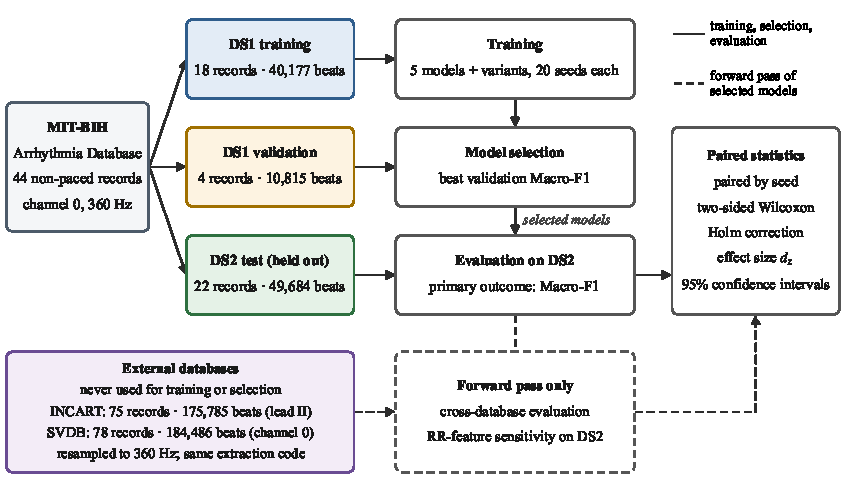
\includegraphics[width=\textwidth]{evaluation_protocol.pdf}
\caption{Evaluation protocol. Training records fit the models, the four validation records determine every checkpoint and configuration choice, and DS2 reports the selected models (DS2 metrics of non-adopted variants were also computed during development; \S\ref{sec:results_selection}). The external databases and the RR-feature sensitivity analysis use forward passes of the selected models only. Counts are read from the split definition and the extraction outputs.}
\label{fig:protocol}
\end{figure}

\begin{table}[!htbp]
\caption{Class distribution and AAMI mapping.}
\label{tab:class_dist}
\centering
\footnotesize
\resizebox{\textwidth}{!}{%
\begin{tabular}{@{}llccccr@{}}
\toprule
\textbf{Class} & \textbf{Included Annotations} & \textbf{Train} & \textbf{Val} & \textbf{Test (DS2)} & \textbf{Total} & \textbf{Ratio (vs N)} \\ \midrule
\textbf{N} & Normal, L, R, e, j & 37,337 & 8,502 & 44,232 & \textbf{90,071} & 1.0 : 1 \\
\textbf{S} & A, a, J, S & 485 & 458 & 1,837 & \textbf{2,780} & 32.4 : 1 \\
\textbf{V} & V, E & 2,321 & 1,467 & 3,220 & \textbf{7,008} & 12.9 : 1 \\
\textbf{F} & F & 28 & 386 & 388 & \textbf{802} & 112.3 : 1 \\
\textbf{Q} & /, f, Q & 6 & 2 & 7 & \textbf{15} & 6,004.7 : 1 \\ \midrule
\textbf{Total} & & \textbf{40,177} & \textbf{10,815} & \textbf{49,684} & \textbf{100,676} & \\ \bottomrule
\end{tabular}%
}
\end{table}

\subsection{PC-WavKAN}
\label{sec:model}
The model (Fig.~\ref{fig:arch}) has a morphology branch and a rhythm branch whose outputs are concatenated and classified.

\begin{figure}[!htbp]
\centering
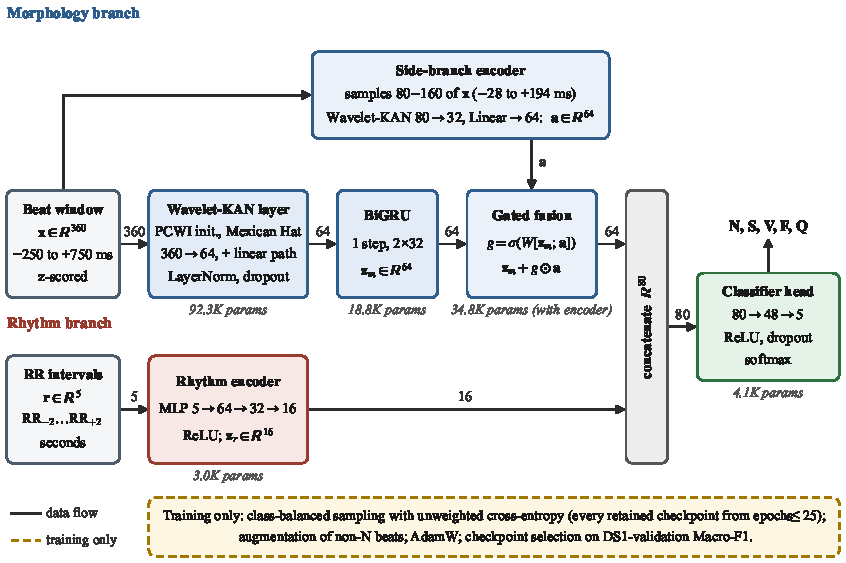
\includegraphics[width=\textwidth]{final_methodology_workflow_v2.pdf}
\caption{PC-WavKAN as implemented, with tensor dimensions and per-block trainable parameters (153,045 in total). Morphology branch: the beat window passes through a wavelet-KAN layer with prior-centred initialisation (PCWI) and a linear residual path, followed by layer normalisation, dropout and a bidirectional GRU applied to a single time step. A side branch encodes raw-beat samples 80--159 (28\,ms before to 192\,ms after the R-peak) into $\mathbf{a}$ with a wavelet-KAN layer, a projection and a single-token attention block; $\mathbf{a}$ is added to the GRU output through a learned sigmoid gate $g$. Rhythm branch: an MLP encodes the five RR intervals. The two branch outputs are concatenated and classified by an $80\rightarrow48\rightarrow5$ head. The mechanisms in the dashed band act during training only.}
\label{fig:arch}
\end{figure}

\paragraph{Wavelet-KAN layer} Following Wav-KAN \cite{bozorgasl_wavkan_2024}, every edge $(j,k)$ carries its own Mexican Hat function $\psi(u) = (1-u^2)e^{-u^2/2}$. The layer maps $x_i \in \mathbb{R}^{360}$ to $\mathbb{R}^{64}$:
\begin{equation}
z^{(k)} = \sum_{j=1}^{360} w_{j,k}\,\psi\!\left(\frac{x_j - \mu_{j,k}}{|\gamma_{j,k}|}\right) + \lambda \sum_{j=1}^{360} v_{j,k}\,x_j, \qquad k = 1,\dots,64,
\label{eq:kan}
\end{equation}
with learnable translation $\mu_{j,k}$, dilation $\gamma_{j,k}$ (the implementation adds $10^{-6}$ to $|\gamma_{j,k}|$) and weight $w_{j,k}$, and a linear residual path with a fixed gate $\lambda = 0.1$, the implementation's default, which was not tuned in this study. $\psi$ is evaluated on the \emph{amplitude} $x_j$ of input sample $j$, so $\mu$ and $\gamma$ are an amplitude offset and an amplitude width. They are not a temporal position or duration. The output is layer-normalised, passed through dropout ($p = 0.2$), and fed to a bidirectional GRU with 32 units per direction. The 64 activations form a single token, so the GRU executes one step in each direction from a zero state. It therefore acts as a gated transformation of the channel vector and integrates no temporal context. It has 18,816 parameters (12.3\% of the model), of which the 6,144 recurrent weights do not affect the output, because they multiply the zero initial state.

\paragraph{Prior-centred wavelet initialisation (PCWI)}
\label{sec:pcwi}
The 64 output channels are split into three blocks, and every edge feeding block $c$ is initialised around a fixed pair $(\bar\mu_c,\bar\gamma_c)$:
\begin{equation}
\mu_{j,k} \sim \mathcal{U}(\bar\mu_c - \epsilon_c,\ \bar\mu_c + \epsilon_c),\qquad
\gamma_{j,k} \sim \mathcal{U}(\bar\gamma_c - \delta_c,\ \bar\gamma_c + \delta_c).
\label{eq:pcwi}
\end{equation}
Channels 1--32 use $(0.0, 0.05)$ with $(\epsilon,\delta) = (0.02, 0.005)$, channels 33--48 use $(-0.10, 0.12)$, and channels 49--64 use $(+0.10, 0.10)$, the last two with $(\epsilon,\delta) = (0.03, 0.01)$. The values were chosen with reference to the relative amplitude and sharpness of the QRS complex and the P and T waves on the $z$-scored scale, and we refer to the blocks by those names (QRS-, P- and T-prior blocks). Without PCWI, all edges use the isotropic initialisation $\mu \sim \mathcal{U}(-0.3, 0.3)$, $\gamma \sim \mathcal{U}(0.05, 0.20)$. The weights $w_{j,k}$ and $v_{j,k}$ use Kaiming-uniform initialisation in both cases.

Two properties limit what PCWI can encode. First, each block's prior is shared by all 360 input samples, so no prior is tied to the temporal location of a waveform component. Second, the 64 channels are exchangeable. They feed a layer normalisation initialised identically across channels and a recurrent layer whose input weights are drawn independently and identically across channels. Permuting the channels together with the corresponding downstream weights leaves the network function unchanged, which we verified numerically (maximum output difference $10^{-7}$). A network in which the P- and T-block priors are exchanged is therefore an exact relabelling of one in which they are not, with the same initial distribution. What PCWI determines is the set of initial $(\mu,\gamma)$ values, 32 channels narrow and centred at zero and 16 each slightly offset and wider, not an assignment of channels to waveform components. We name it \emph{prior-centred} for that reason.

\paragraph{Gated side branch} A side branch reads raw-beat samples 80--159, which with the R-peak at sample 90 spans 28\,ms before to 192\,ms after the R-peak, i.e.\ the QRS complex and early ST segment. The branch was designed to cover the P-wave, which precedes the QRS complex, but its sample range was fixed for an R-peak at sample 180, and it does not reach the P-wave in the window as extracted. We therefore describe it by what it reads. The samples pass through a randomly initialised wavelet-KAN layer ($80\to32$), are projected to 64 dimensions, and pass through a four-head attention block over a single key/value token. With one token the attention softmax is degenerate, so at inference the block is a learned affine map of that token that does not depend on the query; its 8,320 query and key parameters do not affect the output. A sigmoid gate then combines the result with the GRU output. The branch has 34,816 parameters.

\paragraph{Rhythm branch and classifier} The interval vector is encoded to 16 dimensions by a multilayer perceptron (MLP; $5\to64\to32\to16$, ReLU). An alternative encoder that projects each interval to a 16-dimensional token and applies two-head self-attention was also evaluated (\S\ref{sec:results_selection}). The 80-dimensional concatenation is classified by an $80\to48\to5$ head. With the MLP rhythm encoder the model has 153,045 trainable parameters, and 154,325 with the self-attention encoder. Results outside \S\ref{sec:results_selection} use the 153,045-parameter configuration, except three that use the 154,325-parameter base configuration and say so: the pre-specified sampling test (\S\ref{sec:results_sampling}), the interval ablation (\S\ref{sec:results_rr}) and the trained isotropic null (\S\ref{sec:results_ppr}).

\subsection{Training}
\label{sec:training}
Table~\ref{tab:settings} collects the settings. Training uses AdamW (learning rate $10^{-3}$, weight decay $10^{-4}$), batch size 64, gradient-norm clipping at 1.0 and a cosine learning-rate schedule over a nominal 100-epoch budget. Early stopping monitors DS1-validation Macro-F1 with patience 15, and the checkpoint of the best validation epoch is retained. In the 60 class-balanced runs of the three PC-WavKAN configurations whose DS2 results are reported, training stopped between epochs 17 and 40, and at the retained epoch the learning rate had fallen by at most 15\%. The baseline scripts did not log their stopping epoch.

\begin{table}[!htbp]
\centering
\caption{Training and evaluation settings. Every setting above the rule is shared by all five models; the settings below it differ by design (\S\ref{sec:baselines}).}
\label{tab:settings}
\footnotesize
\begin{tabular}{@{}ll@{}}
\toprule
\textbf{Setting} & \textbf{Value} \\ \midrule
Inputs & beat window (360 samples) and five RR intervals \\
Optimiser & AdamW; learning rate $10^{-3}$; weight decay $10^{-4}$ \\
Learning-rate schedule & cosine annealing over a nominal 100 epochs \\
Batch size; gradient clipping & 64; gradient norm 1.0 \\
Early stopping & patience of 15 epochs on DS1-validation Macro-F1 \\
Retained checkpoint & epoch with the best DS1-validation Macro-F1 \\
Seeds & 20, identical for every model (\S\ref{sec:stats}) \\ \midrule
Imbalance handling, PC-WavKAN & class-balanced sampling with unweighted cross-entropy \\
Imbalance handling, baselines & natural sampling; inverse-frequency weighted cross-entropy \\
 & (S weight $\times8$); focal loss without weights for CNN+Focal \\
Augmentation & PC-WavKAN only: non-N beats (noise, baseline wander, scaling) \\ \bottomrule
\end{tabular}
\end{table}

\paragraph{Class-balanced sampling} For the first 25 epochs, mini-batches are drawn by a sampler that selects each class with equal probability, and the loss is unweighted cross-entropy. Each class therefore supplies about one fifth of every mini-batch, so the 6 Q and 28 F training beats are each redrawn many times per epoch. The training script then enters a second phase in which the sampler is annealed towards the natural class distribution and the loss becomes a class-weighted focal loss. In all 60 runs of the three configurations whose DS2 results are reported (20 seeds each), the retained checkpoint came from the first phase (best epochs 2--25), and 20 of these runs stopped before the switch. Of all 160 runs that used this schedule, including the five class-balanced ablation arms of Table~\ref{tab:family_ablation}, 158 retained a first-phase checkpoint; the other two are ablation runs that retained epoch 26 or 27 (Morlet basis, seed 333; no side branch, seed 13). The second phase therefore did not contribute to any model whose DS2 result is reported. We describe and evaluate the procedure by what determined those models: class-balanced sampling with unweighted cross-entropy and validation-based checkpoint selection, abbreviated CBS. The comparator, used by three of the four baselines and by the no-CBS arms, is natural-distribution sampling with inverse-frequency class-weighted cross-entropy, with the S-class weight multiplied by 8. CNN+Focal uses natural-distribution sampling with focal loss and no class weights.

\paragraph{Augmentation} During training only, every non-N beat in a mini-batch is perturbed with probability one. The perturbation is additive Gaussian noise at a 25\,dB signal-to-noise ratio, a sinusoidal baseline wander of 0.5--2.5\,Hz with amplitude 0.01--0.05 (in $z$-units), and amplitude scaling by $\mathcal{U}(0.9, 1.1)$, applied after $z$-scoring. The baselines are trained without augmentation (\S\ref{sec:baselines}).

\subsection{Baselines and What Is Matched}
\label{sec:baselines}
Four architectures spanning 29K--118K parameters are compared (Table~\ref{tab:baselines}). \emph{Held identical:} data, preprocessing, split, input representation (every model receives both the beat window and the interval vector), optimiser, learning rate, weight decay, schedule, epoch budget, early-stopping rule and patience, batch size, gradient clipping, checkpoint-selection rule, the 20 seeds, and, wherever class weights are used, the class-weight formula. \emph{Not held identical:} the imbalance mechanism and augmentation. The baselines use natural-distribution sampling with class-weighted cross-entropy, except CNN+Focal, which uses focal loss without static class weights. We also tested, for the baselines, a class-balanced sampler combined with an inverse-frequency-weighted focal loss. At this imbalance ratio that combination drove the majority-class gradient to near zero, and three of the four baselines then never predicted class N, so it was not used; those runs were not retained. The comparison in \S\ref{sec:results_primary} is therefore between complete methods, i.e.\ architecture together with its imbalance strategy, under a common protocol and budget. \S\ref{sec:results_sampling} and \S\ref{sec:results_augmentation} quantify the two mechanisms on PC-WavKAN itself.

The baseline labelled B-Spline KAN is the same wavelet-KAN layer with a single cubic B-spline in place of the Mexican Hat on every edge, isotropic initialisation, no side branch, no dropout after the layer normalisation, and the same GRU, rhythm MLP and head. It is not the grid-based spline KAN of Liu \emph{et al.} \cite{liu_kan_2024}.

\begin{table}[!htbp]
\caption{Baselines. Protocol, split, inputs, optimiser, budget, checkpoint rule and seeds are identical to PC-WavKAN (\S\ref{sec:baselines}).}
\label{tab:baselines}
\centering
\footnotesize
\resizebox{\textwidth}{!}{%
\begin{tabular}{@{}l r l@{}}
\toprule
\textbf{Model} & \textbf{Params} & \textbf{Imbalance handling} \\ \midrule
ResNet1D (4-block residual CNN, 32 channels) & 62,869 & Weighted cross-entropy \\
Transformer ($d_{\mathrm{model}}{=}32$, 2 layers, 4 heads) & 29,653 & Weighted cross-entropy \\
CNN+Focal (4-layer 1D CNN) & 71,061 & Focal loss ($\gamma{=}2$) \\
B-Spline KAN (single B-spline per edge; no PCWI or side branch) & 118,229 & Weighted cross-entropy \\
\textbf{PC-WavKAN} (\S\ref{sec:model}) & \textbf{153,045} & \textbf{CBS + augmentation} \\ \bottomrule
\end{tabular}%
}
\end{table}

\subsection{Parameter-Space Prior Retention}
\label{sec:ppr_def}
To test RQ3 we measure how close the trained wavelet parameters remain to the PCWI prior values. For block $c$,
\begin{equation}
\mathrm{PPR}_c = \max\!\left(0,\ 1 - \frac{1}{2}\left[\frac{\overline{|\mu_{j,k} - \bar\mu_c|}}{\Delta_\mu} + \frac{\overline{|\,|\gamma_{j,k}| - \bar\gamma_c|}}{\Delta_\gamma}\right]\right),
\label{eq:ppr}
\end{equation}
where the overlines denote means over all edges of block $c$, and $\Delta_\mu = 0.40$, $\Delta_\gamma = 0.20$ are fixed normalising spans. The reported PPR is the unweighted mean over the three blocks. The measure is computed from parameters alone and never observes a model output. The analysis is therefore at the level of basis-function parameters only. It makes no claim about features, attributions or individual predictions, which also pass through the GRU, the side branch, the rhythm branch and the classifier head. Because PCWI initialises at the prior values, an untrained PCWI model scores near-maximally by construction. PPR is therefore interpretable only against reference points, and we report three: untrained with PCWI, untrained with isotropic initialisation, and \emph{trained} with isotropic initialisation. The last one tests whether training moves parameters towards the prior values. Per-edge absolute deviations are averaged rather than block means, because per-edge drift is close to symmetric and largely cancels in the mean (in the trained model, mean per-edge $|\Delta\mu| = 0.064$ against $0.004$ for the deviation of the block means).

\subsection{Statistical Methodology}
\label{sec:stats}
Every arm is trained with the same 20 seeds: 42, 101, 777, 2026, 9999, 1234, 2024, 31415, 27182, 7, 11, 13, 888, 555, 333, 99, 1001, 5050, 8080 and 1998. Comparisons are paired by seed label. Within one architecture, the same seed gives the same initialisation. Across architectures the pairing is by label only and implies no shared initialisation or data order. The signed-rank test remains valid in that case under the null hypothesis of identical distributions. Significance is assessed by the two-sided Wilcoxon signed-rank test \cite{wilcoxon_individual_1945}, with Holm--Bonferroni correction \cite{holm_simple_1979} within declared families. The metrics of one arm-versus-arm comparison form one family, as do the comparisons against the four baselines on one metric, the seven variant-versus-base comparisons of the component ablation, and the five masked positions of the interval ablation. All $p$-values are Holm-adjusted unless labelled raw. Effect sizes are the paired standardised mean difference $d_z = \bar\delta/s_\delta$, reported against Cohen's conventional thresholds \cite{cohen_statistical_1988}: $|d_z| < 0.2$ negligible (negl.), from 0.2 small, from 0.5 medium and from 0.8 large. \textbf{Positive $d_z$ favours PC-WavKAN, the adopted configuration, or the treatment arm.} We also report 95\% confidence intervals on the paired mean difference. The unit of replication is the training seed and the DS2 records are fixed, so the tests and intervals do not include the sampling variability of the 22 test patients. At $n = 20$ and $\alpha = 0.05$ two-sided, a paired $t$-test has 80\% power only for $d_z \gtrsim 0.66$ (slightly more is needed for the signed-rank test), and non-significant results are reported with their intervals rather than as evidence of absence. No equivalence margin was specified, so parity results are not equivalence claims.

\emph{Outcome hierarchy.} Results are reported in \S\ref{sec:results}. The \emph{primary} outcome is DS2 five-class Macro-F1 of the adopted configuration against the four baselines. The \emph{pre-specified secondary} outcome is the effect of the imbalance mechanism on per-class recall, tested on the base configuration (\S\ref{sec:results_sampling}). Everything else is \emph{exploratory}. That includes the same comparison on the adopted configuration, which uses arms trained for the augmentation analysis, and the interval ablation, the cross-database evaluation, the prior-retention analysis and the artefact sensitivity analysis. The last four were added or revised, and the four-class Macro-F1 and a per-record S-recall breakdown were added, after the primary results were known. Exploratory analyses are labelled as such where reported.

\emph{Software.} Models are implemented in PyTorch. Every quantitative claim in this paper is re-derived from the per-seed result files by a verification script released with the code (Code availability).

%% ---------------------------------------------------------------------------
\section{Results}
\label{sec:results}

\subsection{Architecture Selection on Validation Data}
\label{sec:results_selection}
The configuration reported in the rest of this paper is the one that a rule using DS1 validation only selects; when that rule was applied relative to the DS2 results is disclosed under Test-set exposure below. Table~\ref{tab:family_ablation} gives the single-variable ablation. The base configuration has the wavelet-KAN layer with PCWI, the gated side branch, the self-attention rhythm encoder and CBS, and each row changes exactly one component. The validation score of each seed is taken at the epoch its checkpoint was saved.

\begin{table}[!htbp]
\centering
\caption{Single-variable component ablation on \textbf{DS1 validation}, 20 seeds per row. Base configuration: PCWI, gated side branch, self-attention rhythm encoder and CBS; validation Macro-F1 $0.4145\pm0.0201$. $\Delta$ and $d_z$ are variant minus base, so positive values favour the variant. $p$ is Holm-adjusted across the seven comparisons. Removing the side branch also removes 34,816 parameters (22.6\% of the base model). DOG: first derivative of Gaussian.}
\label{tab:family_ablation}
\footnotesize
\resizebox{\textwidth}{!}{%
\begin{tabular}{l c c c c l}
\toprule
\textbf{Variant} & \textbf{Val.\ Macro-F1} & \textbf{$\Delta$ vs base} & \textbf{$d_z$} & \textbf{Holm $p$} & \textbf{Reading} \\ \midrule
No PCWI (isotropic init.) & $0.3932\pm0.0129$ & $-0.0213$ & $-1.05$ (large) & $\mathbf{1{\times}10^{-4}}$ & PCWI helps in this configuration \\
No gated side branch & $0.3976\pm0.0184$ & $-0.0169$ & $-0.54$ (medium) & $0.164$ & not resolved \\
No CBS (reweighting) & $0.4053\pm0.0173$ & $-0.0092$ & $-0.37$ (small) & $0.624$ & not resolved \\
Basis: Morlet & $0.4219\pm0.0187$ & $+0.0074$ & $+0.31$ (small) & $0.568$ & not resolved \\
Basis: DOG & $0.4041\pm0.0123$ & $-0.0104$ & $-0.45$ (small) & $0.164$ & not resolved \\
Basis: B-spline & $0.4116\pm0.0151$ & $-0.0029$ & $-0.14$ (negl.) & $0.624$ & not resolved \\
\textbf{MLP rhythm encoder} & $\mathbf{0.4397\pm0.0140}$ & $\mathbf{+0.0252}$ & $\mathbf{+1.15}$ \textbf{(large)} & $\mathbf{8{\times}10^{-4}}$ & \textbf{adopted} \\ \bottomrule
\end{tabular}%
}
\end{table}

Three findings follow. \emph{Initialisation:} replacing PCWI with the isotropic initialisation costs $0.021$ validation Macro-F1 ($d_z = -1.05$, Holm $p = 1\times10^{-4}$). It is the only component whose removal significantly reduced validation Macro-F1. The comparison contrasts one structured initialisation with one isotropic distribution, and \S\ref{sec:pcwi} shows that what PCWI fixes is a set of amplitude offsets and widths, not a physiological assignment. The finding is therefore that this initialisation helps, not that physiological content does. It was measured in the base configuration and was not re-measured on the adopted configuration. \emph{Mother wavelet:} substituting a Morlet wavelet, the first derivative of Gaussian (DOG) or a B-spline for the Mexican Hat changes validation Macro-F1 by at most $0.010$, and no difference approaches significance. \emph{Rhythm encoder:} replacing self-attention with an MLP over the same five intervals improves validation Macro-F1 by $0.025$ ($d_z = +1.15$, Holm $p = 8\times10^{-4}$). This configuration is the best of all eight on validation. It outperforms each of the seven alternatives (Holm-adjusted $p \leq 0.0032$ over that family), and we adopt it.

\paragraph{Test-set exposure} The adopted configuration was first identified during development, after DS2 metrics of all eight configurations had been computed; at that point the base configuration was known to be significantly below each of the four baselines on DS2 (Holm-adjusted $p \leq 0.005$). The validation analysis of Table~\ref{tab:family_ablation}, carried out afterwards, selects the same configuration, and it is the only selection rule we report. The configuration ranked first on validation is also first of the eight on DS2 ($0.357\pm0.019$; base configuration $0.323\pm0.018$). DS2 was therefore not untouched, and \S\ref{sec:results_primary} should be read as a held-out estimate under a validation-based rule applied after DS2 had been inspected, not as a single-shot test. Any bias from this exposure would favour PC-WavKAN. On arrays regenerated from PhysioNet with the released code, all 20 adopted-configuration checkpoints reproduce their DS2 predictions beat for beat, and 19 reproduce exactly the validation Macro-F1 logged at their saved epoch. Seed 1001's logged validation score does not reproduce. Excluding it changes no corrected conclusion, though the unadjusted interval against B-Spline KAN (Table~\ref{tab:baseline_comparison}) then narrowly excludes zero ($[-0.031, -0.0002]$).

\subsection{Primary Comparison}
\label{sec:results_primary}

\begin{table}[!htbp]
\centering
\caption{\textbf{Primary outcome.} DS2 five-class Macro-F1, PC-WavKAN versus four baselines, 20 paired seeds. $\Delta$, CI and $d_z$ are PC-WavKAN minus baseline; $p$ is Holm-adjusted across the four comparisons.}
\label{tab:baseline_comparison}
\footnotesize
\resizebox{\textwidth}{!}{%
\begin{tabular}{l r c c c c}
\toprule
\textbf{Model} & \textbf{Params} & \textbf{Macro-F1} & \textbf{$\Delta$} & \textbf{95\% CI of $\Delta$} & \textbf{$d_z$ / Holm $p$} \\ \midrule
ResNet1D & 62,869 & $0.351\pm0.019$ & $+0.006$ & $[-0.008, +0.020]$ & $+0.19$ / $1.00$ \\
Transformer & 29,653 & $0.353\pm0.040$ & $+0.004$ & $[-0.013, +0.022]$ & $+0.12$ / $1.00$ \\
CNN+Focal & 71,061 & $0.362\pm0.015$ & $-0.005$ & $[-0.017, +0.006]$ & $-0.22$ / $1.00$ \\
B-Spline KAN & 118,229 & $0.371\pm0.024$ & $-0.014$ & $[-0.029, +0.001]$ & $-0.43$ / $0.36$ \\ \midrule
\textbf{PC-WavKAN} & \textbf{153,045} & $\mathbf{0.357\pm0.019}$ & --- & --- & --- \\ \bottomrule
\end{tabular}%
}
\end{table}

PC-WavKAN's DS2 Macro-F1 is not statistically distinguishable from any baseline (Table~\ref{tab:baseline_comparison}). All Holm-adjusted $p \geq 0.36$, all effects are negligible to small, and every 95\% interval on the paired difference contains zero, the widest bound being $0.029$. The intervals exclude Macro-F1 differences larger than 0.03 in either direction. They do not establish equivalence, for which no margin was set. PC-WavKAN is also the largest of the five models. Because the Q class contributes a near-constant zero (\S\ref{sec:results_perclass}), we also report the four-class N/S/V/F Macro-F1 (exploratory): PC-WavKAN $0.446\pm0.023$, ResNet1D $0.439\pm0.023$, Transformer $0.441\pm0.050$, CNN+Focal $0.453\pm0.019$ and B-Spline KAN $0.463\pm0.030$, with all Holm-adjusted $p \geq 0.36$. The conclusion is unchanged. Removing record 202, the DS2 record from the same subject as training record 201 (\S\ref{sec:split}), lowers every model's Macro-F1 by $0.002$ to $0.006$ (PC-WavKAN: $0.357\rightarrow0.354$), and the comparison is again unchanged: all Holm-adjusted $p \geq 0.25$, and every paired interval lies within $\pm0.03$ (exploratory).

Fig.~\ref{fig:confusion} shows the structure behind these values, averaged over the 20 seeds. N and V separate well, each leaking under 6\% into the other, with V-recall $0.898$. S beats are split almost equally between V ($0.40$) and N ($0.39$), and most F beats are predicted as N ($0.78$).

\begin{figure}[!htbp]
\centering
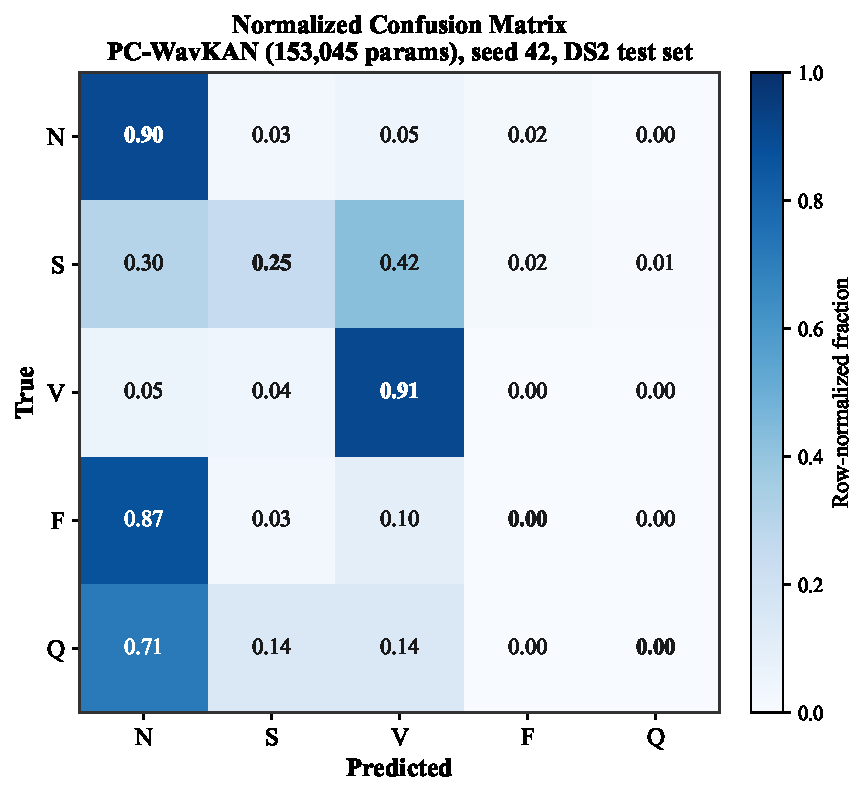
\includegraphics[width=0.75\textwidth]{final_confusion_matrix_main.pdf}
\caption{Row-normalised DS2 confusion matrix of PC-WavKAN, averaged over the 20 seeds. Each seed's matrix is normalised by row and then averaged, and the across-seed standard deviation is shown under each value. Rows are labelled with their support; the Q row rests on 7 beats. The diagonal equals the per-class recall of Table~\ref{tab:perclass}.}
\label{fig:confusion}
\end{figure}

\subsection{Per-Class Operating Points}
\label{sec:results_perclass}
Table~\ref{tab:perclass} gives precision, recall and F1 per class over 20 seeds, recomputed from stored per-seed predictions. The per-class F1 values average to the Macro-F1 of Table~\ref{tab:baseline_comparison} for all five models.

\begin{table}[!htbp]
\centering
\caption{Per-class precision, recall and F1, 20 seeds, DS2. \textbf{(a)} PC-WavKAN, all classes. \textbf{(b)} S class across models, with the Holm-adjusted paired comparison of S-F1 against PC-WavKAN (exploratory; positive $d_z$ favours PC-WavKAN). S-class differences between models combine architecture and imbalance mechanism (\S\ref{sec:baselines}). Q scores exactly zero for every model.}
\label{tab:perclass}
\footnotesize
\begin{tabular}{@{}l c c c c@{}}
\toprule
\multicolumn{5}{@{}l}{\textbf{(a) PC-WavKAN, per class}} \\
\textbf{Class} & \textbf{Support} & \textbf{Precision} & \textbf{Recall} & \textbf{F1} \\ \midrule
N & 44,232 & $0.971\pm0.004$ & $0.905\pm0.025$ & $0.936\pm0.013$ \\
S & 1,837 & $0.175\pm0.079$ & $0.198\pm0.067$ & $0.180\pm0.064$ \\
V & 3,220 & $0.527\pm0.051$ & $0.898\pm0.020$ & $0.663\pm0.039$ \\
F & 388 & $0.005\pm0.006$ & $0.006\pm0.006$ & $0.005\pm0.006$ \\
Q & 7 & $0.000$ & $0.000$ & $0.000$ \\ \midrule
\multicolumn{5}{@{}l}{\textbf{(b) S class across models}} \\
\textbf{Model} & \textbf{S-Prec.} & \textbf{S-Rec.} & \textbf{S-F1} & \textbf{$d_z$ / Holm $p$} \\ \midrule
\textbf{PC-WavKAN} & $0.175$ & $0.198$ & $0.180$ & --- \\
ResNet1D & $0.173$ & $0.100$ & $0.124$ & $+0.77$ / $\mathbf{0.004}$ \\
Transformer & $0.219$ & $0.229$ & $0.207$ & $-0.35$ / $0.312$ \\
CNN+Focal & $0.306$ & $0.075$ & $0.115$ & $+0.85$ / $\mathbf{0.002}$ \\
B-Spline KAN & $0.237$ & $0.280$ & $0.244$ & $-0.66$ / $\mathbf{0.027}$ \\ \bottomrule
\end{tabular}
\end{table}

The S-class operating point is poor in both directions. Recall is $0.198$ at precision $0.175$, so roughly four in five predicted S beats are wrong and four in five true S beats are missed. On S-F1, PC-WavKAN is better than ResNet1D and CNN+Focal, indistinguishable from the Transformer, and worse than B-Spline KAN ($d_z = -0.66$, Holm $p = 0.027$). Its S-recall advantage over ResNet1D and CNN+Focal comes largely from record 232, where those two models detect almost no S beats (Limitation~2). The parity of \S\ref{sec:results_primary} is therefore not uniform across classes. Q contributes an exact zero for every model, consistent with its 6 training beats. With Q at zero, five-class Macro-F1 cannot exceed $0.8$, which should be recalled whenever five-class inter-patient Macro-F1 values are compared.

\paragraph{Comparison with the protocol's source} de Chazal \emph{et al.} \cite{chazal_automatic_2004}, whose partition we adopt, report a sensitivity of $0.759$ at positive predictivity $0.385$ for supraventricular ectopic beats (SVEB, our S class), and $0.777$ at $0.819$ for ventricular ectopic beats (VEB, our V class). On the S class their linear-discriminant system is substantially better than every model trained here on both axes. On the V class our recall of $0.898$ exceeds theirs, while our precision of $0.527$ is lower. Their system uses two leads, hand-engineered morphology at fiducial points and RR-interval features, where ours uses one lead and a fixed window. We have not rerun their method. We report the comparison because the S-class gap is large and is against the protocol's own source.

\subsection{Class-Balanced Sampling Versus Reweighting}
\label{sec:results_sampling}
The pre-specified test compares CBS with reweighting on the base configuration, with augmentation in both arms. S-recall rises from $0.079\pm0.016$ to $0.122\pm0.052$ (Holm $p = 0.0016$ across five metrics, $d_z = +0.77$). On DS1 validation it rises from $0.218\pm0.048$ to $0.305\pm0.047$ ($d_z = +1.36$, raw $p = 2.4\times10^{-4}$). Table~\ref{tab:sampling} repeats the comparison on the adopted configuration. It uses the two augmentation-free arms trained for \S\ref{sec:results_augmentation}, so the analysis is exploratory.

\begin{table}[!htbp]
\caption{CBS versus reweighting on the adopted configuration, both arms without augmentation, 20 paired seeds (exploratory). DS2 rows: $d_z$ and $p$ are CBS minus reweighting, Holm-adjusted across the five metrics. Validation rows: values at each run's retained epoch, raw $p$.}
\label{tab:sampling}
\centering
\footnotesize
\begin{tabular}{@{}l c c c c@{}}
\toprule
\textbf{Metric} & \textbf{Reweighting} & \textbf{CBS} & \textbf{$d_z$} & \textbf{$p$} \\ \midrule
\multicolumn{5}{@{}l}{\emph{DS2 (held out)}} \\
Macro-F1 & $0.351\pm0.014$ & $0.364\pm0.021$ & $+0.52$ (medium) & $0.098$ \\
\textbf{S-Recall} & $\mathbf{0.137\pm0.037}$ & $\mathbf{0.222\pm0.057}$ & $\mathbf{+1.47}$ \textbf{(large)} & $\mathbf{2.9{\times}10^{-5}}$ \\
\textbf{F-Recall} & $\mathbf{0.0003\pm0.0008}$ & $\mathbf{0.0022\pm0.0019}$ & $\mathbf{+0.88}$ \textbf{(large)} & $\mathbf{0.013}$ \\
V-Recall & $0.880\pm0.024$ & $0.880\pm0.017$ & $0.00$ (negl.) & $0.756$ \\
N-Recall & $0.927\pm0.021$ & $0.917\pm0.024$ & $-0.32$ (small) & $0.228$ \\ \midrule
\multicolumn{5}{@{}l}{\emph{DS1 validation}} \\
Macro-F1 & $0.4285\pm0.0125$ & $0.4195\pm0.0098$ & $-0.57$ (medium) & $0.027$ (raw) \\
S-Recall & $0.2639\pm0.0510$ & $0.2391\pm0.0425$ & $-0.53$ (medium) & $0.025$ (raw) \\ \bottomrule
\end{tabular}
\end{table}

On DS2, CBS raises S-recall from $0.137$ to $0.222$, with a 95\% confidence interval of $[+0.058, +0.112]$ on the paired difference. The absolute F-recall gain is negligible ($0.0003\rightarrow0.0022$). V- and N-recall show no corrected change. On the validation partition the direction reverses. CBS is nominally worse on both validation Macro-F1 and S-recall, although after Holm correction across the two validation metrics neither difference is significant ($p \approx 0.05$). The DS2 gain in S-recall therefore replicates in two configurations but is not reproduced on the four-record validation partition for the adopted configuration. We read this as indicating that the benefit of class-balanced sampling for supraventricular beats may depend on the patients evaluated, and we do not claim it as a general property. The pre-specified test on the base configuration is the confirmatory evidence, and it is modest in absolute terms: an S-recall of $0.122$.

\subsection{Augmentation}
\label{sec:results_augmentation}
PC-WavKAN is trained with minority-class augmentation and the baselines are not; this analysis is exploratory. On validation, augmentation is supported: with CBS in both arms, it raises validation Macro-F1 by $0.020$ ($d_z = +1.16$, raw $p = 1.7\times10^{-4}$), consistent with its place in the adopted recipe. On DS2, removing it leaves Macro-F1 statistically unchanged ($0.357$ with augmentation and $0.364$ without; Holm $p = 0.46$ across four metrics) and reduces F-recall ($0.0061$ to $0.0022$, Holm $p = 0.043$). The augmentation asymmetry therefore does not explain the parity in Table~\ref{tab:baseline_comparison}. A separate, shorter study used a different recipe: 60 epochs with patience 12, class-balanced sampling combined with class-weighted cross-entropy throughout, and noise settings that differ from the adopted augmentation. In it, the three noise-based strategies raised V-recall and lowered Macro-F1, and a SMOTE-style interpolation \cite{chawla_smote_2002}, which replaces each minority beat by a random convex combination of it and a random beat of the same class in the mini-batch (possibly itself), produced the largest S-recall gain ($0.316 \rightarrow 0.648$) at the largest Macro-F1 cost. The Macro-F1 penalty of the noise-based strategies did not carry over to the full recipe, which cautions against extrapolating short single-mechanism ablations.

\subsection{Interval Features, Lookahead and an Annotation-Derived Artefact}
\label{sec:results_rr}
An exploratory leave-one-out analysis set each interval position in turn to 0.8\,s at inference. It used the base configuration, whose rhythm features are identical to the adopted one's, with 20 seeds, two-sided tests and Holm correction across the five positions. Masking $RR_0$ caused by far the largest loss of S-recall ($-0.0323\pm0.0492$, Holm $p = 6\times10^{-4}$). This is expected, since an ectopic beat that fires early shortens its preceding interval, the classical sign of prematurity. Masking $RR_{+2}$ caused a small loss that survives correction ($-0.0045\pm0.0103$, Holm $p = 0.028$). The other three positions had no corrected effect. The model therefore draws signal from an interval that has not elapsed when beat $i$ occurs, which is one reason we treat the task as offline (\S\ref{sec:preprocessing}).

\paragraph{Annotation-derived artefact} Because the intervals are computed between consecutive annotation-file entries, including non-beat markers, 4,578 of 49,684 DS2 beats (9.2\%) have at least one interval that differs from the beat-to-beat value, and 1,433 (2.9\%) have a different $RR_0$. By class, $RR_0$ differs for 6.4\% of V beats, against 2.7\% of N beats and 1.3\% of S beats, and the recorded value is almost always shorter than the true interval, which mimics prematurity. A rhythm-change marker is placed where an arrhythmic episode begins, so this artefact carries annotation-derived information that would not be available on unannotated recordings, and it correlates with the label. We quantified its effect without retraining, as an exploratory analysis. We recomputed every DS2 interval between beat annotations only and re-evaluated all 100 published checkpoints (five models, 20 seeds). The recomputation leaves the beats and their order unchanged. As a check, the same re-evaluation with the published intervals reproduced every model's reported Macro-F1. Of the 100 checkpoints, 88 reproduced every DS2 prediction exactly. The remaining 12, all CNN+Focal, differed in 1 to 4 of 49,684 beats, which we attribute to floating-point differences between the original GPU inference and the re-evaluation (TF32 disabled; deterministic algorithms not enforced). With beat-to-beat intervals, the Macro-F1 of every model rose slightly, in all 20 seeds. The mean increase was $+0.002$ to $+0.005$ across the five models (PC-WavKAN: $0.357\rightarrow0.360$), and PC-WavKAN's V-recall changed by $-0.001$. The primary comparison was unchanged: all Holm-adjusted $p \geq 0.38$, and every paired interval still includes zero. The artefact therefore did not inflate the reported performance, and removing it at inference does not change the comparative conclusions. The models were trained with it, and whether training on beat-to-beat intervals would change them was not tested.

\subsection{Retention of the Prior Values}
\label{sec:results_ppr}
Table~\ref{tab:ppr} evaluates PPR against its three reference points (exploratory).

\begin{table}[!htbp]
\centering
\caption{Parameter-space Prior Retention \eqref{eq:ppr}, mean$\pm$std over 20 models, with mean absolute per-edge deviations from the prior values. Untrained rows use 20 initialisation seeds. The trained isotropic row uses the 20 checkpoints of the no-PCWI ablation arm (base configuration).}
\label{tab:ppr}
\footnotesize
\begin{tabular}{l c c c}
\toprule
\textbf{Model state} & \textbf{PPR} & $\overline{|\Delta\mu|}$ & $\overline{|\Delta\gamma|}$ \\ \midrule
Untrained, PCWI & $0.9729\pm0.0001$ & $0.013$ & $0.004$ \\
\textbf{Trained, PCWI (PC-WavKAN)} & $\mathbf{0.7826\pm0.0351}$ & $0.064$ & $0.055$ \\
Untrained, isotropic & $0.6698\pm0.0008$ & $0.161$ & $0.051$ \\
Trained, isotropic & $0.5794\pm0.0173$ & $0.177$ & $0.080$ \\ \bottomrule
\end{tabular}
\end{table}

Training moves the PCWI parameters substantially: PPR falls from $0.973$ to $0.783$, and the mean per-edge translation deviation grows fivefold. The trained PCWI basis nonetheless remains closer to the prior values than an untrained isotropic basis ($0.783$ against $0.670$). The trained isotropic row decides the interpretation. When training starts from the isotropic initialisation, it moves the parameters \emph{further} from the prior values ($0.670 \rightarrow 0.579$). Both comparisons separate the 20 models completely (two-sided Mann--Whitney test, raw $p = 7\times10^{-8}$ by the normal approximation). Training from the isotropic initialisation therefore does not lead towards the prior values. The trained PCWI model's proximity to them reflects where it started, not a learned preference. Together with the exchangeability of the channel blocks (\S\ref{sec:pcwi}), this means the wavelet parameters of this model do not support a physiological interpretation. They support the modest statement that the initial structure is partly retained. Fig.~\ref{fig:wavelets} shows the per-edge parameters behind these values. The retention lies mainly in the translations, which stay centred on the prior values. The dilations of the P- and T-prior blocks spread to a distribution broadly similar to that of the isotropic arm. Automated interpretability metrics for sparse autoencoders can score randomly initialised transformers similarly to trained ones \cite{heap_automated_2025}, and our results indicate that parameter-space scores for KANs need the same reference points.

\begin{figure}[!htbp]
\centering
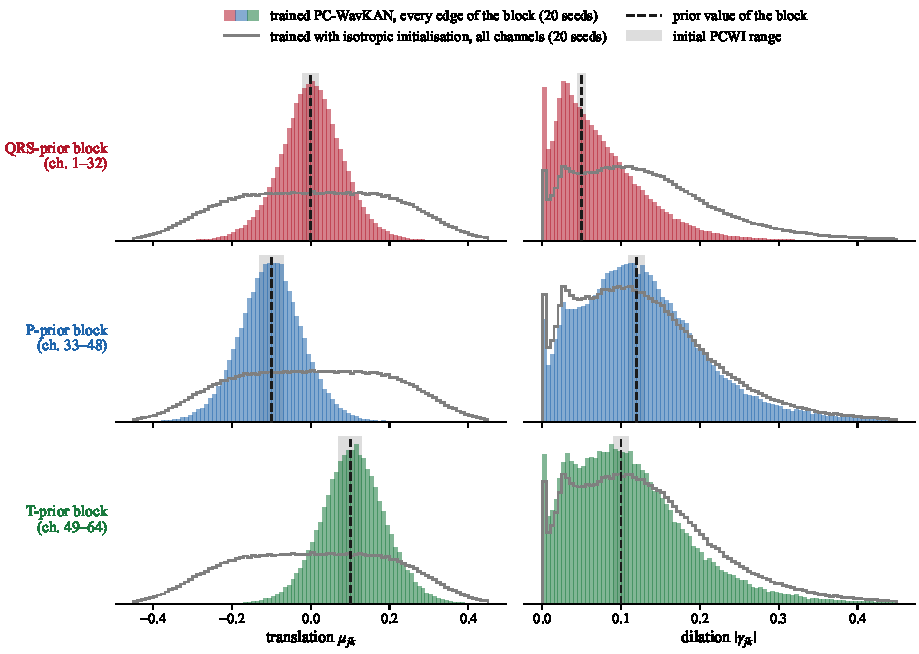
\includegraphics[width=\textwidth]{final_learned_wavelets.pdf}
\caption{Per-edge wavelet parameters after training. Coloured histograms pool every edge of each channel block over all 20 seeds of PC-WavKAN. They are shown against the block's prior value (dashed line) and initial PCWI range (grey band), and against the trained isotropic-initialisation arm of the base configuration, all channels (grey outline; the trained null of Table~\ref{tab:ppr}). Histograms are normalised to unit area. Translations stay centred on the prior values but spread well beyond their initial range. The dilations of the P- and T-prior blocks spread to a distribution broadly similar to the null's. Block names refer to initial values, not to functions.}
\label{fig:wavelets}
\end{figure}

\subsection{Cross-Database Evaluation}
\label{sec:results_crossdata}
Table~\ref{tab:multidataset} evaluates the five models trained on MIT-BIH on two further databases, forward pass only, 20 seeds each. The first is the St Petersburg INCART 12-lead Arrhythmia Database \cite{goldberger_physiobank_2000, pollard_physionet_2026}, all 75 records, lead II. The second is the MIT-BIH Supraventricular Arrhythmia Database (SVDB) \cite{greenwald_improved_1990}, 78 records, channel 0, whose leads are not labelled. Both were resampled to 360\,Hz and then passed through a re-implementation of the training extraction. A regression test confirms that it gives output byte-identical to the training extraction on MIT-BIH records, and the DS2 arrays it regenerates are identical to the training-pipeline arrays. Neither database was used for any training, tuning or selection decision. SVDB was assembled to enrich supraventricular ectopy and serves as an S-class stress test. The analysis is exploratory.

\begin{table}[!htbp]
\centering
\caption{Zero-shot cross-database evaluation under the training preprocessing, 20 seeds per model. $d_z$ and $p$ compare PC-WavKAN with each baseline on Macro-F1 (positive favours PC-WavKAN), Holm-adjusted within each database; bold marks Holm $p<0.05$.}
\label{tab:multidataset}
\footnotesize
\resizebox{\textwidth}{!}{%
\begin{tabular}{l c c c c c c c c}
\toprule
& \multicolumn{4}{c}{\textbf{INCART} (175,785 beats)} & \multicolumn{4}{c}{\textbf{SVDB} (184,486 beats)} \\
\cmidrule(lr){2-5}\cmidrule(lr){6-9}
\textbf{Model} & \textbf{Macro-F1} & \textbf{$d_z$ / Holm $p$} & \textbf{V-Rec.} & \textbf{S-Rec.} & \textbf{Macro-F1} & \textbf{$d_z$ / Holm $p$} & \textbf{V-Rec.} & \textbf{S-Rec.} \\ \midrule
\textbf{PC-WavKAN} & $0.390\pm0.017$ & --- & $0.832$ & $0.671$ & $0.275\pm0.012$ & --- & $0.788$ & $0.126$ \\
ResNet1D & $0.431\pm0.017$ & $-1.80$ / $\mathbf{<0.001}$ & $0.849$ & $0.760$ & $0.350\pm0.026$ & $-2.49$ / $\mathbf{<0.001}$ & $0.832$ & $0.256$ \\
Transformer & $0.398\pm0.032$ & $-0.24$ / $0.245$ & $0.852$ & $0.817$ & $0.316\pm0.031$ & $-1.36$ / $\mathbf{<0.001}$ & $0.820$ & $0.305$ \\
CNN+Focal & $0.431\pm0.020$ & $-1.53$ / $\mathbf{<0.001}$ & $0.807$ & $0.560$ & $0.354\pm0.013$ & $-4.86$ / $\mathbf{<0.001}$ & $0.769$ & $0.179$ \\
B-Spline KAN & $0.367\pm0.017$ & $+0.83$ / $\mathbf{0.003}$ & $0.820$ & $0.606$ & $0.267\pm0.016$ & $+0.33$ / $0.231$ & $0.791$ & $0.125$ \\ \bottomrule
\end{tabular}%
}
\end{table}

PC-WavKAN shows no transfer advantage. On INCART its Macro-F1 of $0.390$ is significantly below ResNet1D and CNN+Focal (both $0.431$; $d_z \leq -1.53$, Holm $p < 0.001$). It is indistinguishable from the Transformer and above B-Spline KAN ($d_z = +0.83$, Holm $p = 0.003$). On SVDB it is significantly below all three non-KAN baselines (Holm $p < 0.001$) and indistinguishable from B-Spline KAN, and the two KAN-family models have the lowest Macro-F1 of the five. Fig.~\ref{fig:forest} places the in-distribution and cross-database comparisons on one scale.

\begin{figure}[!htbp]
\centering
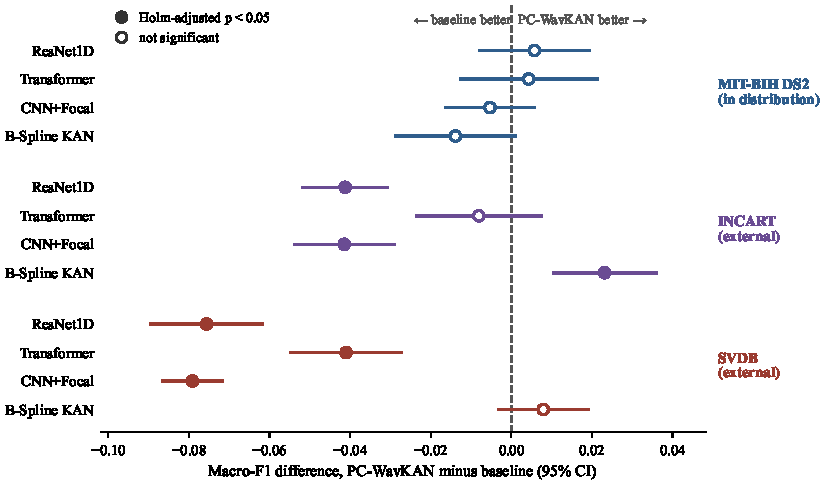
\includegraphics[width=0.873\textwidth]{macro_f1_forest.pdf}
\caption{Paired Macro-F1 differences, PC-WavKAN minus each baseline, with 95\% confidence intervals over 20 seeds. The three groups cover MIT-BIH DS2 (Table~\ref{tab:baseline_comparison}) and the two external databases (Table~\ref{tab:multidataset}). Filled markers indicate Holm-adjusted $p<0.05$ across the four baselines within a database; the dashed line marks zero. In distribution, every interval includes zero. Out of distribution, PC-WavKAN is below both convolutional baselines.}
\label{fig:forest}
\end{figure}

On SVDB, both KAN-family models also have the highest S$\rightarrow$V confusion rates ($0.431$ and $0.451$, mean over seeds, against $0.231$--$0.395$ for the other models) and assign the largest share of beats to V ($18.7\%$ and $20.7\%$, against $8.4$--$17.6\%$). We report this as a descriptive pattern; the study does not identify its cause.

\paragraph{Sensitivity to preprocessing} An earlier evaluation of the same checkpoints used windows from only 30 INCART records, on lead I, and applied no filter. It ranked PC-WavKAN first on INCART (Macro-F1 $0.374$ against $0.316$--$0.365$ for the baselines). Matching the preprocessing to the training data reversed that ranking. Cross-database comparisons of this kind are therefore sensitive to preprocessing details that are not always reported, and we report only the matched evaluation.

\subsection{Efficiency}
\label{sec:results_deploy}
Table~\ref{tab:deployment} reports inference on an x86 CPU for the seed-42 checkpoint, on random inputs and with PyTorch's default thread count. Values are the mean of three repeated runs, each of 1000 timed trials at batch 1 (200 at batch 64) after a 20-iteration warm-up, and $\pm$ is the standard deviation across the three runs.

\begin{table}[!htbp]
\centering
\caption{Measured inference, PC-WavKAN, x86 CPU, PyTorch 2.6. Sizes are in MiB.}
\label{tab:deployment}
\footnotesize
\begin{tabular}{l c}
\toprule
\textbf{Metric} & \textbf{Value} \\ \midrule
Model size, FP32 / INT8 dynamic & $0.596$ / $0.551$ MiB ($1.08\times$) \\
Latency, batch 1, FP32 & $2.93\pm0.38$ ms/beat (median $2.78$) \\
Latency, batch 1, INT8 dynamic & $4.00\pm0.35$ ms/beat ($0.73\times$, slower) \\
Latency, batch 64, FP32 & $0.429$ ms/beat \\
Process resident memory after benchmarking & $235$ MiB \\ \bottomrule
\end{tabular}
\end{table}

Dynamic INT8 quantisation brings no benefit and slows inference. It was applied to the \texttt{nn.Linear} modules, which hold 11.4\% of the parameters; the custom wavelet-KAN layers and the GRU, which hold 77.5\%, remain in FP32. The FP32 latency supports continuous offline processing on a general-purpose CPU. We made no ARM or on-device measurement and make no claim about wearable deployment.

%% ---------------------------------------------------------------------------
\section{Discussion}
\label{sec:discussion}

\paragraph{What the study shows} Under a matched protocol with multiplicity control, the wavelet KAN is not statistically distinguishable from four standard architectures on Macro-F1, with every paired interval within $\pm0.03$. It is not more accurate than a 30K-parameter Transformer, and we do not present the wavelet-KAN basis as an accuracy mechanism. Among its design choices, in the configuration in which components were ablated, initialising the wavelet parameters in a structured, prior-centred way helped relative to an isotropic initialisation, and the choice of mother wavelet did not measurably matter. The inspectability argument for wavelet KANs does not transfer to a physiological reading of this model's parameters. The channel blocks are exchangeable, and training moves unconstrained parameters away from the prior values, not towards them. An inspectable parameter is not thereby an interpretable one. A claim that such parameters encode physiology would need behavioural evidence, for example a selective loss of one class when one block's functions are perturbed. The null models we report are the minimum needed to interpret a parameter-space score.

\paragraph{Self-attention over interval features} Removing self-attention from the rhythm encoder improved validation Macro-F1 with a large effect, while \S\ref{sec:results_rr} shows that the interval features carry real signal, concentrated in $RR_0$. The deficit therefore appears to lie in the encoder rather than in the features. One structural property of the evaluated encoder is consistent with this. Every interval is embedded by the same affine map, and the attention block has no residual connection. Whatever the weights, each output token of the block is therefore an affine function of two attention-weighted averages of the five intervals, one per head. The value of $RR_0$ enters those averages only in proportion to the attention it receives, and otherwise acts only through the attention weights, which depend on interval values rather than positions because the encoder has no positional encoding. The MLP receives the five intervals directly. We did not test whether this property causes the loss, and we observed the loss in one architecture and one dataset.

\paragraph{The external evaluation qualifies the parity} Under preprocessing matched to training, the wavelet KAN transferred worse than both convolutional baselines on both external databases, and the two KAN-family models were the weakest on SVDB. In this study, therefore, the parameterisation that is inspectable in principle came with no accuracy advantage in distribution and a disadvantage out of distribution. Anyone choosing an architecture for data from other sources should weigh the second against the first. The earlier, unmatched evaluation that appeared to show the opposite on INCART is a concrete example of how a preprocessing mismatch can manufacture an apparent transfer advantage.

\subsection{Limitations}
\label{sec:limitations}
\noindent\textbf{(1) Parity, not advantage or equivalence.} No equivalence margin was set. The 95\% intervals are compatible only with Macro-F1 differences within roughly $\pm0.03$, and they describe variation over training seeds on the fixed DS2 records, not over patients.

\noindent\textbf{(2) Absolute minority-class performance.} S-recall is $0.198$ at precision $0.175$. F-recall is below 0.01 for every model and configuration (PC-WavKAN: $0.006$), reflecting 28 training beats. Q, with 6 training beats, supports no per-class conclusion and adds a near-constant zero to the five-class average. One DS2 record, 232, holds 1,382 of the 1,837 S beats (75\%), so the DS2 S-class results largely reflect a single patient. In an exploratory breakdown over 20 seeds, PC-WavKAN's S-recall is 0.138 on record 232 and 0.380 on the 455 S beats of the other records; every model is lower on record 232, where ResNet1D and CNN+Focal detect almost none of the S beats (0.004 and 0.013).

\noindent\textbf{(3) Selection history of the test set.} The adopted configuration is the one a validation-based rule selects, but it was first adopted after the DS2 metrics of all eight configurations had been seen, and the rule was formalised afterwards.

\noindent\textbf{(4) Scope of the component evidence.} Every component ablation, including PCWI, was run on the base configuration. The adopted configuration differs from it only in the rhythm encoder, and no other component was re-ablated on it. We do not claim that PCWI improves the adopted model.

\noindent\textbf{(5) Validation partition.} Validation comprises four records, and one record holds 90\% of DS1's fusion beats. Selection decisions and the validation reversal in Table~\ref{tab:sampling} should be read with that in mind.

\noindent\textbf{(6) Non-causal inputs and an annotation-derived artefact.} The inputs include two following intervals, a window that often contains the next beat, and a zero-phase record-level filter. The interval features also carry an annotation-derived artefact in 9.2\% of DS2 beats. Its effect is bounded in \S\ref{sec:results_rr}. It was not removed by retraining.

\noindent\textbf{(7) External data.} Cross-database evidence rests on two databases. INCART is evaluated on lead II rather than MIT-BIH's modified lead II, and SVDB's leads are unlabelled. PTB-XL \cite{wagner_ptb-xl_2020} was processed but is excluded. Its labels are record-level, not beat-level. Our extraction used a symmetric window with the R-peak at sample 180 rather than 90, no filter, R-peaks from a peak detector rather than expert annotations, and interval features expressed as ratios to a local 10-beat mean rather than in seconds. A Macro-F1 of $0.200\pm0.005$ was obtained, and we attribute it to these mismatches rather than to transfer.

\noindent\textbf{(8) Baselines and hardware.} The baselines were trained without PC-WavKAN's class-balanced sampler and augmentation (\S\ref{sec:baselines}), so the parity is between complete methods, and a common imbalance recipe could change the comparison. The B-Spline KAN baseline is a single-bump variant, not a grid-based spline KAN. Latency is x86 CPU only.

\paragraph{Future work} The results point to three specific questions: whether a causal variant (preceding intervals only, a truncated window and a causal filter) preserves the parity; whether the wavelet-KAN family's behaviour holds on 12-lead recordings with beat-level labels; and whether any behavioural test links individual wavelet parameters to class-specific evidence.

%% ---------------------------------------------------------------------------
\section{Conclusion}
\label{sec:conclusion}
We evaluated a 153,045-parameter wavelet Kolmogorov--Arnold network for inter-patient ECG heartbeat classification under the de Chazal protocol, with 20 paired seeds, multiplicity correction, effect sizes, confidence intervals and a validation-based architecture selection rule, applied after DS2 had been inspected. Its DS2 Macro-F1 of $0.357\pm0.019$ is not statistically distinguishable from four standard baselines of 29K--118K parameters, and all five models share a poor supraventricular operating point. In the configuration in which components were ablated, structured initialisation of the wavelet parameters helped relative to an isotropic one, the mother wavelet did not measurably matter, and self-attention over interval features was harmful. The parameters do not support a physiological reading once exchangeability and a trained null are considered. Class-balanced sampling raised DS2 supraventricular recall but not on the validation partition. Under preprocessing matched to training, the wavelet KAN transferred worse than both convolutional baselines to INCART and SVDB. We report these null and negative findings alongside the positive ones because, on this evidence, they are the more transferable part of what the study found.

%% ---------------------------------------------------------------------------
\section*{CRediT authorship contribution statement}
\textbf{Venkateramanan Manivannan:} Conceptualization, Methodology, Software, Validation, Formal analysis, Investigation, Data curation, Writing -- original draft, Visualization. \textbf{Ramanathan Lakshmanan:} Conceptualization, Resources, Validation, Supervision, Project administration, Funding acquisition, Writing -- review \& editing.

\section*{Declaration of competing interest}
The authors declare that they have no known competing financial interests or personal relationships that could have appeared to influence the work reported in this paper.

\section*{Funding}
The Vellore Institute of Technology (VIT) funds the article processing charge. This research received no other specific grant.

\section*{Ethics statement}
This study uses only publicly available, de-identified PhysioNet databases \cite{goldberger_physiobank_2000, pollard_physionet_2026}. No new human-subject data were collected, and no institutional review board approval was required.

\section*{Data availability}
All datasets are publicly available from PhysioNet \cite{goldberger_physiobank_2000, pollard_physionet_2026}: the MIT-BIH Arrhythmia Database \cite{moody_impact_2001} (\url{https://physionet.org/content/mitdb/1.0.0/}), the St Petersburg INCART 12-lead Arrhythmia Database (\url{https://physionet.org/content/incartdb/1.0.0/}), the MIT-BIH Supraventricular Arrhythmia Database \cite{greenwald_improved_1990} (\url{https://physionet.org/content/svdb/1.0.0/}) and PTB-XL \cite{wagner_ptb-xl_2020} (\url{https://physionet.org/content/ptb-xl/1.0.3/}).

\section*{Code availability}
\url{https://github.com/vrhsr/WavKAN-CL} contains the source code, preprocessing and training scripts, statistical and figure code, the per-seed test metrics of every arm reported here, the training histories and confusion matrices of every PC-WavKAN arm, the per-seed confusion matrices of all five models from the inference-only re-evaluations, the 20 checkpoints of the evaluated PC-WavKAN configuration, and the 20 checkpoints of its isotropic-initialisation ablation arm used for the prior-retention null. Baseline checkpoints are available from the authors on request. \texttt{src/verify\_manuscript\_numbers.py} re-derives the quantitative claims of this manuscript from those files. The repository name is historical.

\section*{Declaration of generative AI and AI-assisted technologies in the manuscript preparation process}
During the preparation of this work the authors used Claude (Anthropic) in order to assist with writing and code development. After using this tool, the authors reviewed and edited the content as needed and take full responsibility for the content of the published article.

\bibliographystyle{elsarticle-num}
\bibliography{references}

\end{document}
